\section{Lösungskonzept}
Dieses Kapitel beinhaltet die Beschreibung der Architektur udn wichtiger Komponenten. Die eingesetzten Technologien und genauen Implementationsdetails stehen im Hintergrund und werden im Kapitel 4 aufgegriffen. Neben der Architektur beinhaltet das Lösungskonzept auch eine allgemeine Schnittstellenbeschreibung. Informationen zur technischen Anbindung an die Schnittstellen können im Abschnitt 7 \tbd im Anhang entnommen werden.

\subsection{Allgemeine Systemsicht}
Anhand der Problembeschreibung wurde ein Plan erarbeitet, der das ganze System verständlich beschreibt. Abbildung \ref{fig:systemView} stellt die wichtigsten Komponenten und Entitäten aus der Problemdomäne in gegenseitiger Beziehung dar.

\begin{figure}[h!]
	\centering
		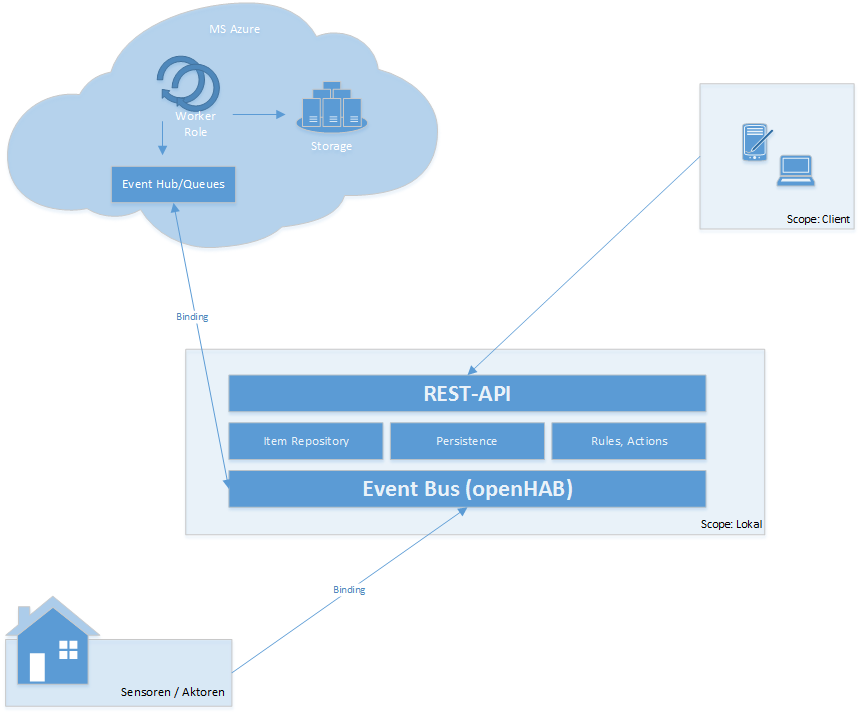
\includegraphics[scale=0.55]{report/img/systemuebersicht}
	\caption{Systemübersicht}
	\label{fig:systemView}
\end{figure}